\documentclass[tikz,border=15pt]{standalone}
\usepackage{amsmath,amssymb}
\usetikzlibrary{patterns}

\begin{document}
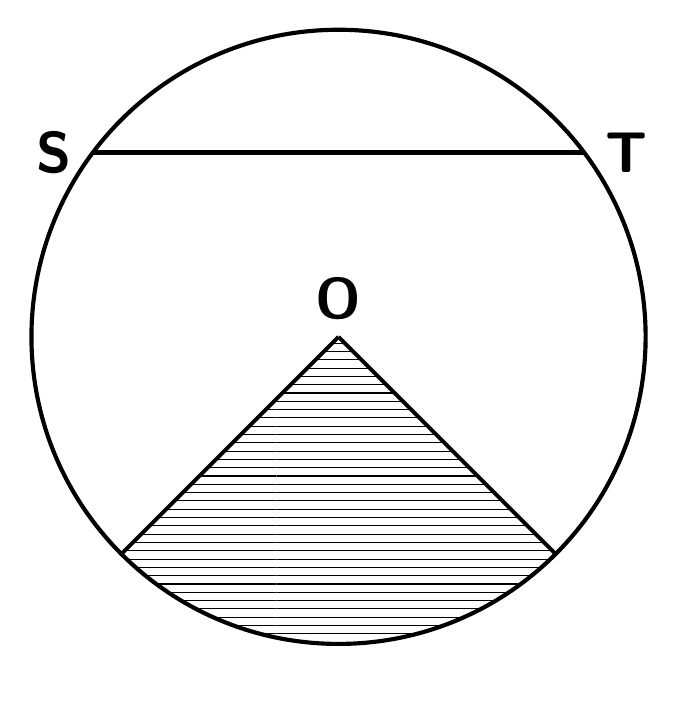
\begin{tikzpicture}[scale=1.3]
    \def\r{3.0} % circle radius
    \def\yChord{1.8}
    \pgfmathsetmacro{\xChord}{sqrt(\r*\r - \yChord*\yChord)} % exactly 2.4
    
    \coordinate (O) at (0, 0);
    \coordinate (S) at (-\xChord, \yChord);
    \coordinate (T) at (\xChord, \yChord);
    
    % Shaded sector in the bottom quadrant (from -135 to -45, span 90 deg)
    \fill[pattern=horizontal lines, pattern color=black] (O) -- (-135:\r) arc (-135:-45:\r) -- cycle;
    \draw[line width=1.4pt] (O) -- (-135:\r);
    \draw[line width=1.4pt] (O) -- (-45:\r);
    
    % Circle boundary
    \draw[line width=1.5pt] (O) circle (\r);
    
    % Horizontal chord ST
    \draw[line width=1.5pt] (S) -- (T);
    
    % Labels
    \node[above=3pt, font=\huge\sffamily\bfseries] at (O) {O};
    \node[left=4pt, font=\huge\sffamily\bfseries] at (S) {S};
    \node[right=4pt, font=\huge\sffamily\bfseries] at (T) {T};
    
\end{tikzpicture}
\end{document}
